\documentclass{beamer}

\usepackage{verbatim}
%\usepackage{verbatimbox}
\usepackage{parskip}
\usepackage{geometry}
\usepackage[colorlinks=true]{hyperref}
%\usepackage{csquotes}
%\usepackage{framed}

\title{Open Source Software for Social \& Scientific Research}
\author{Dr. M. Kamakshaiah \\ Assistant Professor - Business Analytics, \\ GSIB - GITAM \tiny{(Deemed to be University)} \\ \small{kamakshaiah.musunuru@gitam.edu} \\ \vspace{2cm} 
\includegraphics[height=1cm, width=1cm]{gitam_logo} 
\includegraphics[height=1cm, width=1cm]{gsib_logo}}



\date{}

\begin{document}
\titlepage 
\newpage
\tableofcontents

\begin{frame}
\centering 
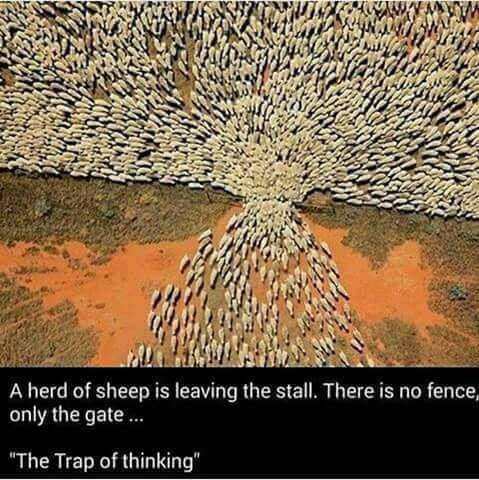
\includegraphics[width=10cm, height=8cm]{goats}
\end{frame}


\section{GUI Based}

\subsection{Spreadsheet Applications}

\begin{frame}{Libre Office Suite}
\centering 
	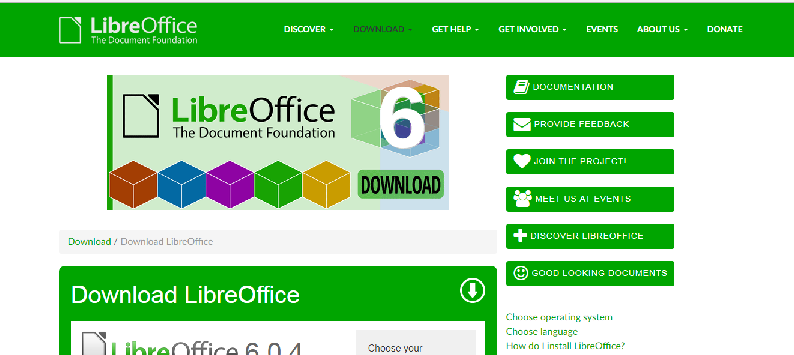
\includegraphics[height=5cm, width=9cm]{lo}
\end{frame}

\begin{frame}{LO Calc - Spreadsheet Application}
\centering 
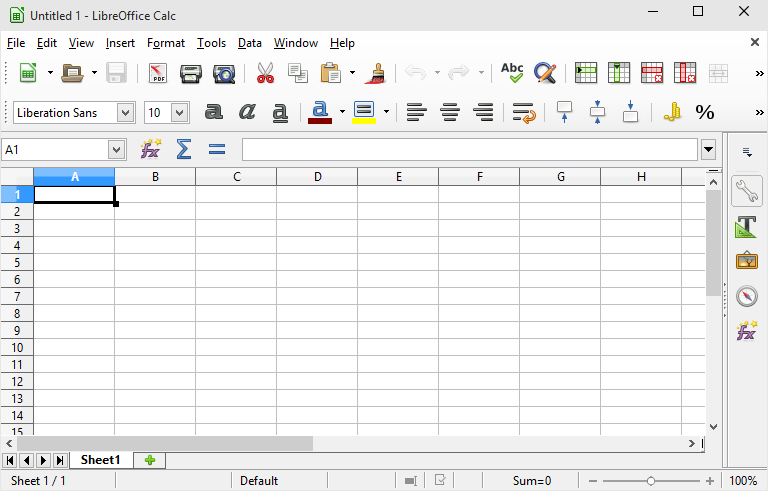
\includegraphics[height=7cm, width=11cm]{lo_calc}
HOME - \url{https://www.libreoffice.org/download/download/}
\end{frame}

\begin{frame}{Gnumeric - GNU Office Suite}
\centering 
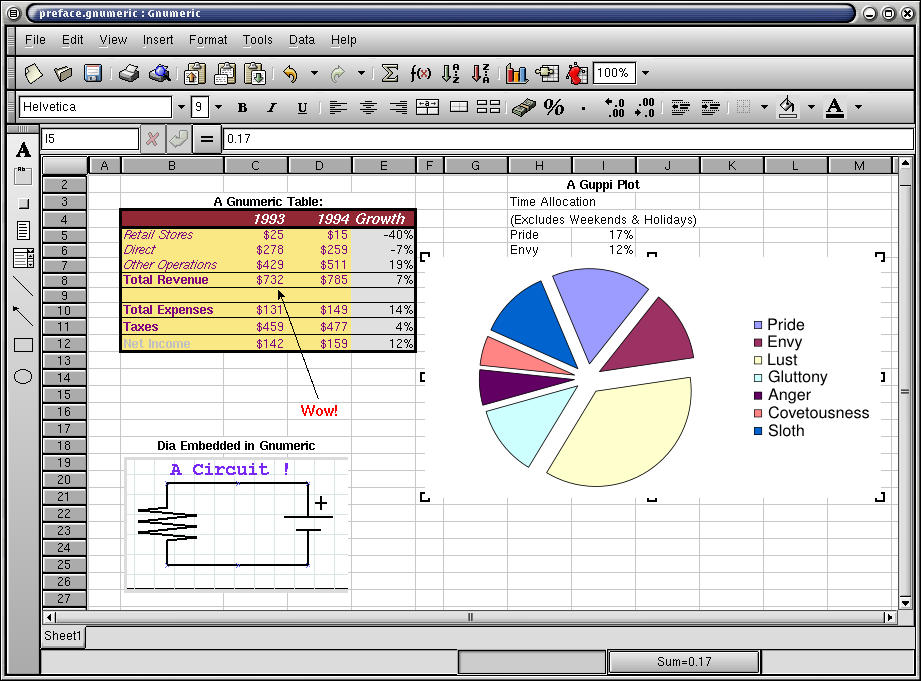
\includegraphics[height=7cm, width=11cm]{gnumeric}
Download - \url{https://sourceforge.net/projects/gnumericportabl/files/latest/download?source=directory}
\end{frame}

\begin{frame}{Pyspread}
\centering 
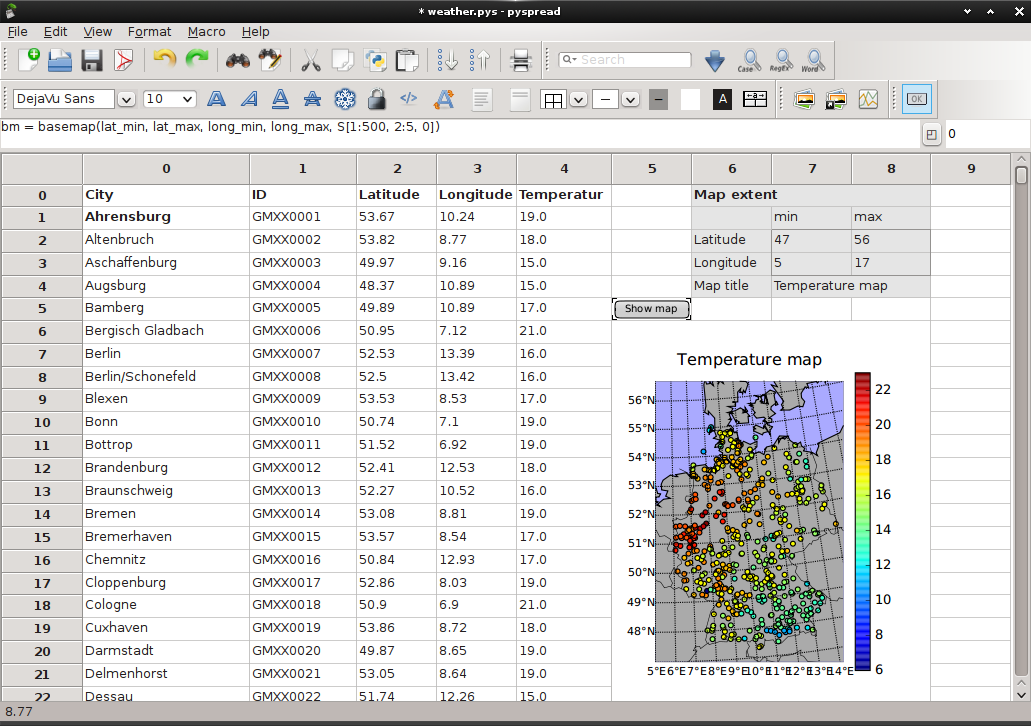
\includegraphics[height=6cm, width=10cm]{pyspread}

HOME - \url{https://manns.github.io/pyspread/}
\end{frame}

\subsection{SPSS like software?}

\subsubsection{PSPP}

\begin{frame}{PSPP}
	\begin{enumerate}
		\item Open source alternative to SPSS. 
		\item GUI based drop-down menus (useful for editing, coding, transforming, analysis and reports). 

	\end{enumerate}
	
For HOME - \url{https://www.gnu.org/software/pspp/get.html} \\ \vspace{1cm}
To Download - \url{http://pspp.awardspace.com/}	
\end{frame}

\begin{frame}{PSPP}
\centering 
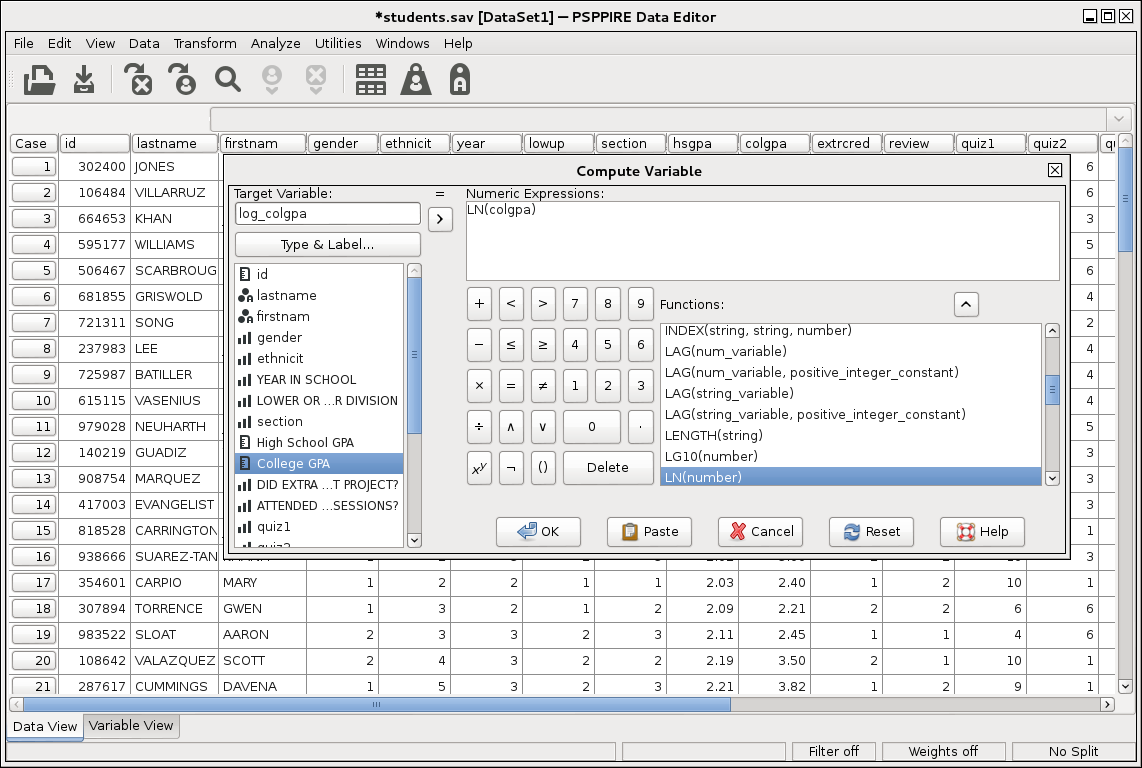
\includegraphics[height=7cm, width=11cm]{pspp}
\end{frame}

\subsubsection{JASP}

\begin{frame}{JASP}
\centering 
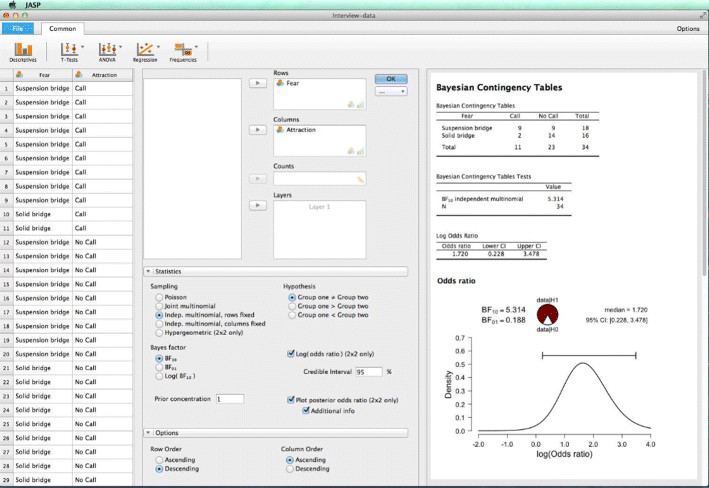
\includegraphics[height=7cm, width=11cm]{jasp}
HOME - \url{https://jasp-stats.org/download/}
\end{frame}

\section{CUI Based Applications}

\subsection{GNU/R}

\begin{frame}{R}
\centering 
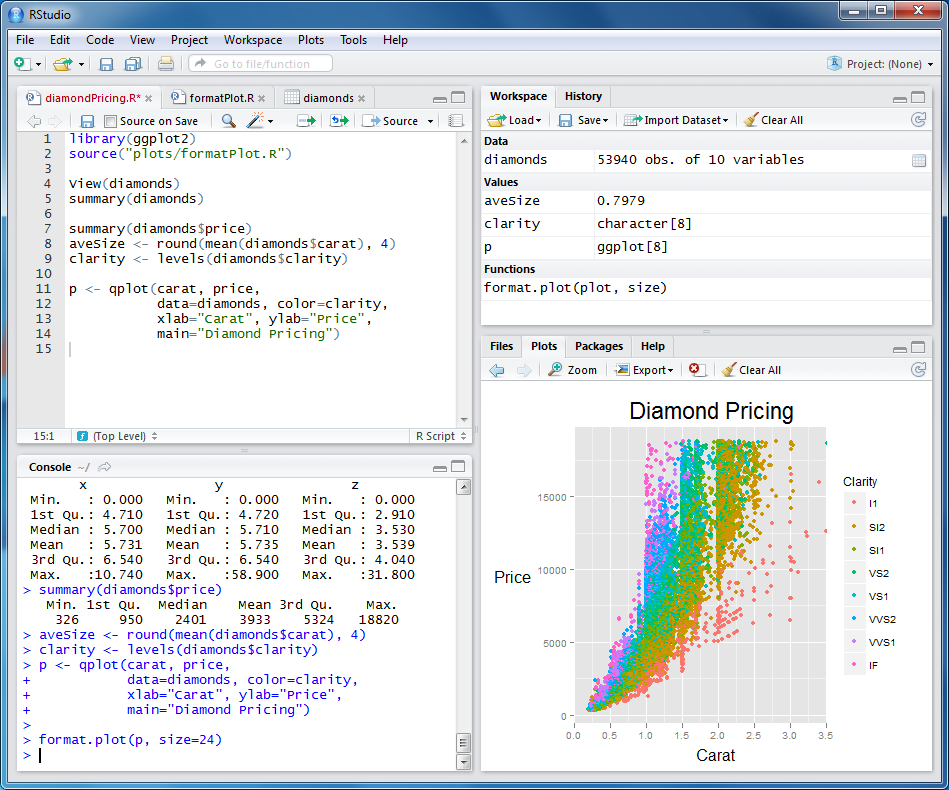
\includegraphics[height=7cm, width=11cm]{r}

R - \url{https://jasp-stats.org/download/} \\ \vspace{0.5cm}
RStudio - \url{https://www.rstudio.com/}

\end{frame}

\subsection{Python}

\begin{frame}{Python}
\centering 
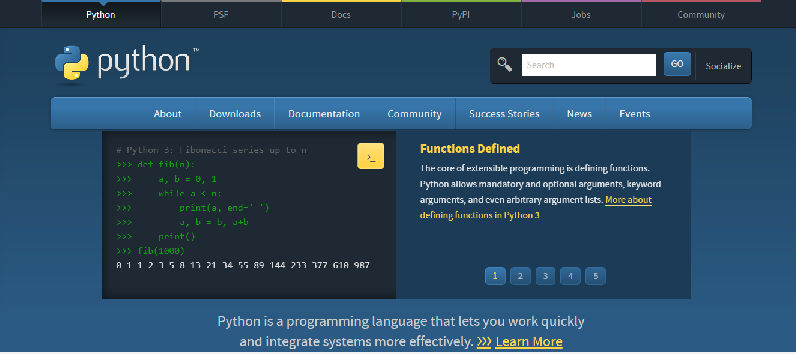
\includegraphics[height=7cm, width=11cm]{python}

HOME - \url{https://www.python.org/} 
\end{frame}

\begin{frame}{Spyder}
\centering 
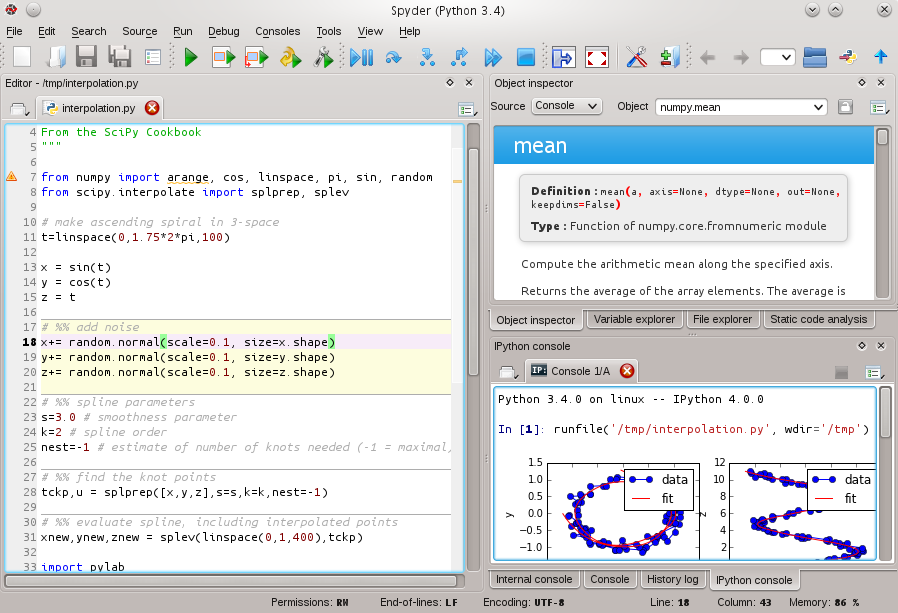
\includegraphics[height=7cm, width=11cm]{spyder}
\end{frame}

\section{Onyx}

\section{Advanced Tools for SEM}

\begin{frame}{Onyx for SEM}
\centering 
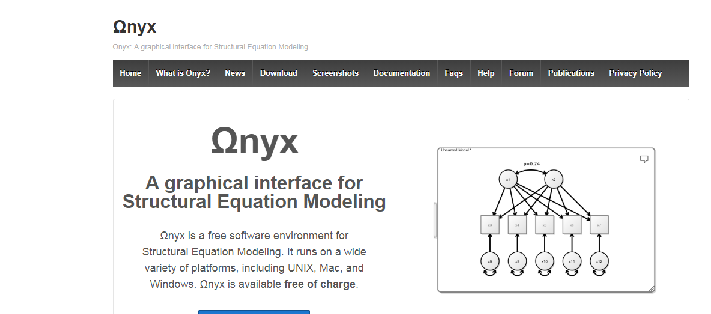
\includegraphics[height=5cm, width=11cm]{onyx_1}
HOME - \url{http://onyx.brandmaier.de/}
\end{frame} 

\begin{frame}{Onyx for SEM}
\centering 
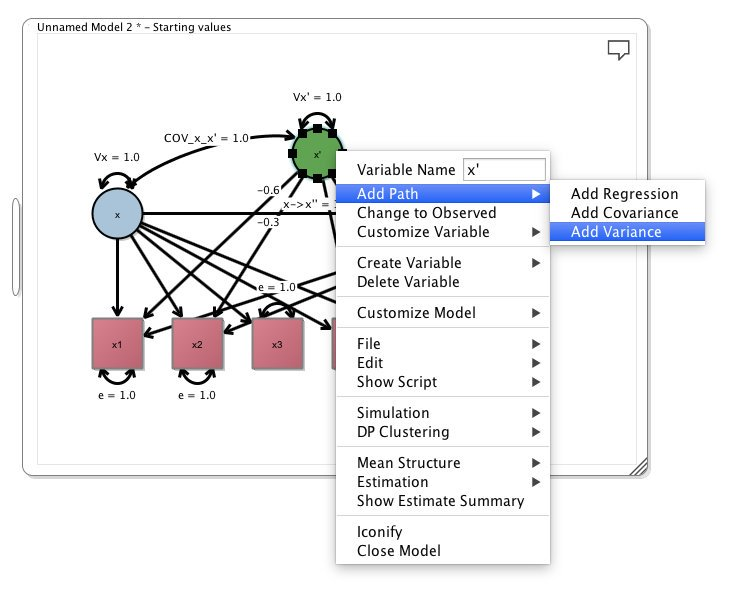
\includegraphics[height=7cm, width=11cm]{onyx.jpg}

\end{frame} 


\begin{frame}

\centering 


\includegraphics[height=2cm, width=2cm]{gnu}

\includegraphics[height=1cm, width=4cm]{fsf}

\includegraphics[height=2cm, width=1.5cm]{wiki}

USE OPEN SOURCE SOFTWARE, \\
REMAIN AS ETHICAL ACADEMIC, \\
LIVE WITH FREEDOM...

Please visit -

\url{https://www.gnu.org/links/links.en.html}
\url{https://www.fsf.org/}
\url{https://www.wikipedia.org/}

\end{frame}








\end{document}